\chapter{Sprint 1 : Authentification et Gestion Multi-Tenant}

\section*{Introduction}

Ce chapitre présente la réalisation du premier sprint de TalentFlow, en lien avec les
user stories US01 à US03 du backlog produit (chapitre~2). Ce sprint constitue le socle
fondamental de la plateforme : il couvre la mise en place du modèle multi-tenant initial,
les mécanismes d'authentification et d'inscription des acteurs Candidat, Tenant et
Administrateur, ainsi que le développement de l'espace d'administration. Nous présentons
successivement l'objectif du sprint, son backlog, l'analyse des cas d'utilisation associés,
puis les interfaces réalisées.

% ============================================================
\section{Objectif du Sprint}
% ============================================================

L'objectif principal de ce sprint est de mettre en place les fondations de la plateforme
TalentFlow en implémentant :

\begin{itemize}
    \item Le \textbf{modèle multi-tenant initial} : entités \texttt{Tenant} et
    \texttt{Entreprise} liées par \texttt{TenantId}, avec statuts
    (\texttt{Pending}, \texttt{Approved}, \texttt{Rejected}) et contrôle d'accès à la
    connexion pour les recruteurs.

    \item Un \textbf{système d'authentification unifié} (inscription, connexion JWT,
    OAuth) pour les profils Candidat, Tenant (recruteur) et Administrateur.

    \item Le \textbf{flux de validation des tenants} par l'administrateur avant
    l'accès à l'espace recruteur.

    \item L'\textbf{espace d'administration} : tableau de bord, validation des demandes
    d'inscription, gestion des tenants approuvés (consultation, suspension) et paramètres
    du compte administrateur.
\end{itemize}

% ============================================================
\section{Analyse du Sprint 1}
% ============================================================

\subsection{Sprint Backlog}

Le tableau~\ref{tab:backlog_s1} présente les user stories réalisées durant ce sprint.

\begin{table}[h]
\centering
\renewcommand{\arraystretch}{1.4}
\begin{tabular}{|c|p{8.5cm}|c|}
\hline
\textbf{ID} & \textbf{User Story} & \textbf{Priorité} \\
\hline
US01 & En tant qu'administrateur, je veux mettre en place l'infrastructure multi-tenant
afin de gérer plusieurs sociétés indépendamment (entités \texttt{Tenant}, \texttt{Entreprise},
statuts et isolation par tenant). & Haute \\
\hline
US02 & En tant qu'utilisateur, je veux accéder à une page d'accueil présentant la
plateforme TalentFlow avec les options de connexion et d'inscription. & Haute \\
\hline
US03 & En tant que candidat, je veux m'inscrire sur la plateforme en renseignant mes
informations personnelles afin d'accéder à mon espace dédié. & Haute \\
\hline
US04 & En tant que tenant, je veux m'inscrire en soumettant les informations de mon
entreprise (nom, RNE, email professionnel, secteur), sachant que mon compte sera soumis
à validation avant activation. & Haute \\
\hline
US05 & En tant qu'utilisateur, je veux me connecter à la plateforme via mes identifiants
ou via un fournisseur OAuth (Google, LinkedIn, Facebook) afin d'accéder à mon espace. & Haute \\
\hline
US06 & En tant qu'administrateur, je veux consulter le tableau de bord d'administration
avec les demandes d'inscription des tenants et les indicateurs clés de la plateforme. & Haute \\
\hline
US07 & En tant qu'administrateur, je veux consulter le détail d'une demande tenant et
l'approuver ou la rejeter afin de contrôler l'accès à la plateforme. & Haute \\
\hline
US08 & En tant qu'administrateur, je veux accéder à la page de gestion des tenants
approuvés avec leurs informations et statistiques, et suspendre un tenant si nécessaire. & Haute \\
\hline
US09 & En tant qu'administrateur, je veux gérer les paramètres de mon compte (profil,
sécurité, préférences de notifications) depuis l'espace administration. & Moyenne \\
\hline
\end{tabular}
\caption{Sprint Backlog du Sprint 1}
\label{tab:backlog_s1}
\end{table}

\subsection{Diagramme de Cas d'Utilisation — Sprint 1}

\begin{figure}[ht]
    \centering
    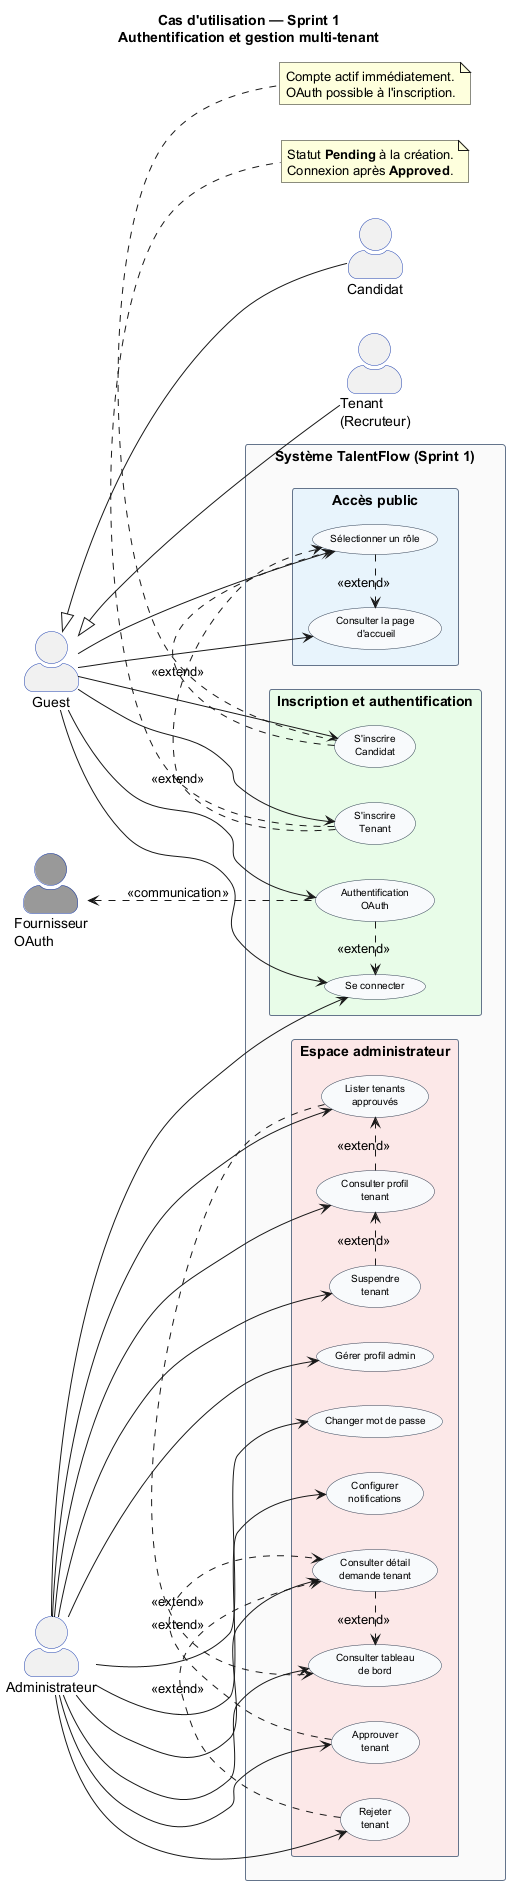
\includegraphics[width=\textwidth]{images/usecase_sprint1.png}
    \caption{Diagramme de cas d'utilisation du Sprint 1}
    \label{fig:uc_sprint1}
\end{figure}

\subsubsection{Description Textuelle des Cas d'Utilisation}

\textbf{Cas d'utilisation : S'inscrire en tant que Candidat}

\begin{itemize}
    \item \textbf{Acteur principal :} Candidat
    \item \textbf{Précondition :} l'utilisateur n'a pas encore de compte.
    \item \textbf{Scénario nominal :}
    \begin{enumerate}
        \item L'utilisateur accède à la page d'accueil et clique sur \textit{Get Started}.
        \item Il sélectionne le rôle \textit{Candidate} puis \textit{Get Started}, ou
        accède directement au formulaire candidat.
        \item Il renseigne son nom complet, son email professionnel, son mot de passe
        et la confirmation, \textbf{ou} s'authentifie via LinkedIn, Google ou Facebook
        (OAuth).
        \item Il clique sur \textit{Create Candidate Profile}.
        \item Le système crée les entités \texttt{Utilisateur} (rôle \texttt{Candidat})
        et \texttt{Candidat}, puis redirige vers l'espace candidat après connexion.
    \end{enumerate}
    \item \textbf{Postcondition :} le compte candidat est créé et actif immédiatement
    (\texttt{TenantStatus} non applicable).
\end{itemize}

\textbf{Cas d'utilisation : S'inscrire en tant que Tenant}

\begin{itemize}
    \item \textbf{Acteur principal :} Tenant (entreprise)
    \item \textbf{Précondition :} l'utilisateur n'a pas encore de compte entreprise.
    \item \textbf{Scénario nominal :}
    \begin{enumerate}
        \item L'utilisateur sélectionne le rôle \textit{Company} et clique sur
        \textit{Hire Talent}.
        \item Il renseigne le nom de l'entreprise, le nom du responsable (CEO), le RNE,
        l'email professionnel, le mot de passe et le secteur d'activité.
        \item Il accepte les conditions d'utilisation et soumet le formulaire
        (\textit{Create Account}) — inscription par email/mot de passe uniquement
        (pas d'OAuth sur ce formulaire).
        \item Le système crée \texttt{Utilisateur} (rôle \texttt{Tenant}),
        \texttt{Tenant} (statut \texttt{Pending}) et \texttt{Entreprise}, puis affiche
        un message de soumission en attente de validation.
    \end{enumerate}
    \item \textbf{Postcondition :} le tenant est en attente (\texttt{Pending} en base ;
    affiché \textit{Pending Review} dans l'interface admin).
    \item \textbf{Exception :} le tenant ne peut pas se connecter tant que le statut
    n'est pas \texttt{Approved}.
\end{itemize}

\textbf{Cas d'utilisation : Valider un Tenant (Admin)}

\begin{itemize}
    \item \textbf{Acteur principal :} Administrateur
    \item \textbf{Précondition :} une demande d'inscription est en statut \texttt{Pending}.
    \item \textbf{Scénario nominal :}
    \begin{enumerate}
        \item L'administrateur consulte le tableau de bord et voit les demandes en attente.
        \item Il clique sur l'icône de consultation pour voir les détails de l'entreprise
        (RNE, secteur, responsable, email, date de création).
        \item Il clique sur \textit{Approve} pour valider ou \textit{Reject} pour refuser.
        \item Le statut du tenant passe à \texttt{Approved} ou \texttt{Rejected}.
    \end{enumerate}
    \item \textbf{Postcondition :} le tenant approuvé peut se connecter et accéder à
    l'espace recruteur (\texttt{/recruiter/dashboard}).
\end{itemize}

\textbf{Cas d'utilisation : Suspendre un Tenant approuvé (Admin)}

\begin{itemize}
    \item \textbf{Acteur principal :} Administrateur
    \item \textbf{Précondition :} le tenant est en statut \texttt{Approved}.
    \item \textbf{Scénario nominal :}
    \begin{enumerate}
        \item L'administrateur ouvre la page \textit{Tenant Management}.
        \item Il consulte la fiche d'un tenant approuvé et confirme l'action
        \textit{Suspend tenant}.
        \item Le système met à jour le statut du tenant (rejet/suspension) via l'API
        \texttt{PATCH /api/admin/tenants/\{rne\}/suspend}.
    \end{enumerate}
    \item \textbf{Postcondition :} le tenant ne peut plus accéder normalement à la plateforme.
\end{itemize}

% ============================================================
\section{Réalisation}
% ============================================================

\subsection{Page d'Accueil}

La page d'accueil de TalentFlow (\texttt{WelcomePage.vue}) constitue le point d'entrée
de la plateforme (route \texttt{/}). Elle présente le positionnement de la solution —
\textit{« Revolutionize Your Recruitment with AI-Powered Intelligence »} — accompagné
d'une illustration du tableau de bord. Deux boutons principaux sont proposés :
\textit{Login} pour les utilisateurs existants et \textit{Get Started} pour les
nouveaux utilisateurs, redirigés vers la sélection du rôle.

\begin{figure}[ht]
    \centering
    \includegraphics[width=\textwidth]{images/welcomepage.jpg}
    \caption{Page d'accueil de TalentFlow}
    \label{fig:welcomepage}
\end{figure}

\subsection{Inscription — Sélection du Rôle}

Lorsqu'un nouvel utilisateur clique sur \textit{Get Started}, il est dirigé vers la page
de sélection du rôle (\texttt{RoleSelection.vue}). Deux options lui sont proposées :
\textbf{Candidate} (personnes en recherche d'emploi) et \textbf{Company} (entreprises
souhaitant recruter), avec les actions \textit{Get Started} et \textit{Hire Talent}
respectivement.

\begin{figure}[ht]
    \centering
    \includegraphics[width=\textwidth]{images/registerpage.jpg}
    \caption{Page de sélection du rôle lors de l'inscription}
    \label{fig:registerpage}
\end{figure}

\subsection{Inscription Candidat}

Le formulaire d'inscription candidat (\textit{Join the Talent Pool}, \texttt{RegisterCandidate.vue})
collecte le nom complet, l'email, le mot de passe et la confirmation. L'utilisateur peut
également s'inscrire via LinkedIn, Google ou Facebook lorsque les fournisseurs OAuth sont
configurés côté serveur (\texttt{appsettings.SocialAuth.json}). Une fois le formulaire
soumis, le compte est créé et activé immédiatement.

\begin{figure}[ht]
    \centering
    \includegraphics[width=0.7\textwidth]{images/registercandidat.jpg}
    \caption{Formulaire d'inscription candidat}
    \label{fig:registercandidat}
\end{figure}

\subsection{Inscription Tenant (Entreprise)}

Le formulaire d'inscription tenant (\textit{Register your company}, \texttt{RegisterCompany.vue})
collecte les informations de l'entreprise : nom de la société, nom du responsable (CEO),
RNE, email professionnel, mot de passe et secteur d'activité. Le compte est créé avec le
statut \texttt{Pending} : une modale confirme que l'inscription est \textit{under review}
et l'entreprise ne peut pas se connecter tant que l'administrateur n'a pas approuvé la demande.

\begin{figure}[ht]
    \centering
    \includegraphics[width=0.7\textwidth]{images/registercomp.jpg}
    \caption{Formulaire d'inscription tenant (entreprise)}
    \label{fig:registercomp}
\end{figure}

\subsection{Page de Connexion}

La page de connexion (\texttt{Login.vue}) est commune aux acteurs Candidat, Tenant et
Administrateur. Elle propose une authentification par email et mot de passe. L'option
\textit{Keep me logged in} est affichée à titre ergonomique ; la session repose sur le
stockage du token JWT côté navigateur. L'authentification OAuth (Google, Facebook,
LinkedIn) redirige vers \texttt{/auth/callback} après traitement par l'API .NET.
Un lien \textit{Forgot password?} est présent dans l'interface mais n'est pas encore
branché à un flux de réinitialisation dans cette version.

\begin{figure}[ht]
    \centering
    \includegraphics[width=0.7\textwidth]{images/login.jpg}
    \caption{Page de connexion unifiée}
    \label{fig:login}
\end{figure}

\subsection{Tableau de Bord Administrateur}

Le tableau de bord administrateur (\textit{Admin portail}, \texttt{TenantRequests.vue})
constitue le centre de contrôle de la plateforme. Il affiche la liste des demandes de
validation d'entreprises (\textit{Company Validation Requests}), avec pour chaque entrée :
le nom de la société, le RNE, le propriétaire, le domaine, le statut (\textit{Approved},
\textit{Rejected}, \textit{Pending Review}) et les actions (Approve, Reject, Consultation).

En bas de page, deux widgets complètent le tableau de bord : un graphique des nouvelles
inscriptions de tenants sur les 5 derniers jours, et un panneau \textit{Infrastructure
Health} (tenants enregistrés, offres actives, demandes en attente, nouveaux tenants sur
24~h).

\begin{figure}[ht]
    \centering
    \includegraphics[width=\textwidth]{images/dashboardadmin.jpg}
    \caption{Tableau de bord administrateur}
    \label{fig:dashboardadmin}
\end{figure}

\subsection{Consultation des Détails d'une Demande Tenant}

Depuis le tableau de bord, l'administrateur peut consulter le détail d'une demande
d'inscription. Une fenêtre modale affiche les informations complètes de l'entreprise :
nom, statut courant, identifiant, RNE, secteur, responsable, email et date de création.
Les boutons \textit{Approve} et \textit{Reject} permettent de statuer sur la demande
(\texttt{PATCH} sur les endpoints \texttt{/api/admin/tenant-requests/...}).

\begin{figure}[ht]
    \centering
    \includegraphics[width=0.75\textwidth]{images/consultation.jpg}
    \caption{Fenêtre de consultation des détails d'une demande tenant}
    \label{fig:consultation}
\end{figure}

\subsection{Gestion des Tenants Approuvés}

La page \textit{Tenant Management} (\texttt{TenantManagement.vue}) offre une vue globale
sur les tenants approuvés. Quatre indicateurs sont affichés en en-tête : tenants approuvés,
offres actives, industries représentées et nouveaux tenants du mois. La liste est filtrable
par secteur et triable par nom. Chaque carte présente le profil du recruteur et de
l'entreprise associée.

\begin{figure}[ht]
    \centering
    \includegraphics[width=\textwidth]{images/tenantmanagement.jpg}
    \caption{Page de gestion des tenants approuvés}
    \label{fig:tenantmanagement}
\end{figure}

\subsection{Suspension d'un Tenant}

Depuis la fiche détaillée d'un tenant approuvé, l'administrateur peut déclencher
l'action \textit{Suspend tenant}. Après confirmation, l'API
\texttt{PATCH /api/admin/tenants/\{rne\}/suspend} met à jour le statut du tenant,
empêchant la poursuite de l'activité sur la plateforme. Cette fonctionnalité complète
la validation initiale en offrant un levier de modération post-approbation.

\subsection{Consultation du Profil Complet d'un Tenant}

En cliquant sur la consultation d'une carte tenant, l'administrateur accède au profil
détaillé dans une fenêtre modale : sections \textit{Contact \& Présence} (téléphone,
site web, LinkedIn, Twitter/X, email) et \textit{Organization} (entreprise, RNE, secteur,
offres actives, date d'approbation, statut de recrutement).

\begin{figure}[ht]
    \centering
    \includegraphics[width=0.75\textwidth]{images/consultationtenant.jpg}
    \caption{Consultation du profil complet d'un tenant}
    \label{fig:consultationtenant}
\end{figure}

\subsection{Paramètres du Compte Administrateur}

L'espace \textit{Settings} (\texttt{AdminSettings.vue}) est organisé en trois onglets :

\textbf{Profile :} modification des informations personnelles (prénom, nom, email,
téléphone, rôle/département) et sauvegarde via \texttt{PUT /api/admin/profile}.

\begin{figure}[ht]
    \centering
    \includegraphics[width=\textwidth]{images/settings1.jpg}
    \caption{Paramètres administrateur — Onglet Profil}
    \label{fig:settings1}
\end{figure}

\textbf{Security :} changement du mot de passe (mot de passe actuel, nouveau mot de passe,
confirmation) via \texttt{POST /api/admin/change-password}.

\begin{figure}[ht]
    \centering
    \includegraphics[width=\textwidth]{images/settings2.jpg}
    \caption{Paramètres administrateur — Onglet Sécurité}
    \label{fig:settings2}
\end{figure}

\textbf{Notifications :} configuration des préférences par interrupteurs (file de validation
des entreprises, décisions d'onboarding, digest plateforme, alertes sécurité). L'interface
permet de régler ces options ; la persistance métier des préférences pourra être étendue
dans une évolution ultérieure.

\begin{figure}[ht]
    \centering
    \includegraphics[width=\textwidth]{images/settings3.jpg}
    \caption{Paramètres administrateur — Onglet Notifications}
    \label{fig:settings3}
\end{figure}

\section*{Conclusion}

Ce premier sprint a posé les fondations essentielles de TalentFlow. Le système
d'authentification multi-rôles (Candidat, Tenant, Administrateur) a été implémenté,
avec inscription OAuth pour les candidats et connexion OAuth pour tous les profils.
Le flux de validation des tenants (\texttt{Pending} $\rightarrow$ \texttt{Approved} ou
\texttt{Rejected}) garantit le contrôle de l'accès des entreprises. L'espace
d'administration — tableau de bord, validation des demandes, gestion et suspension des
tenants approuvés, paramètres du compte admin — offre une visibilité et des leviers de
modération adaptés. Le modèle multi-tenant initial (\texttt{Tenant}, \texttt{Entreprise},
\texttt{TenantId}) constitue le socle sur lequel reposent les sprints suivants, notamment
l'espace tenant et la gestion des experts (chapitre~4).
